%===============================================================
% CHAPTER 4 - Detailed Concept Design (All Five Phases)
%===============================================================
\chapter{Detailed Concept Design}
\label{sec:detailed-concept-design}

This chapter presents the five-phase concept design process for the Solift H-VTOL. The discussion follows the project evidence from solar-cell testing, wing and airfoil selection, CAD modelling, payload-fixture design, foldable propeller development, and tilt-rotor integration. Each phase keeps the same practical focus: the aircraft should not only look plausible in CAD, but also remain manufacturable, inspectable, and testable with the tools available to the team.

\section{Phase 1: Feasibility analysis}
\label{subsec:phase1-feasibility}

The feasibility analysis for Solift considers whether the five main design areas can be developed into a manufacturable aircraft concept within the limits of the course. The analysis is divided into technical, economic, schedule, and operational feasibility, but these categories are closely connected. A design that is technically possible may still be unsuitable if it requires expensive tooling, too much assembly time, or a level of precision that cannot be reached with the available manufacturing process. For Solift, the feasibility question is not only whether the aircraft can fly in theory. The more useful question is whether its solar surface, wing, fixture, foldable propeller, and tilt mechanism can be made and assembled in a controlled way by a small team.

The solar cell subsystem is technically feasible because it is based on a commercial monocrystalline silicon photovoltaic cell rather than a custom cell design. The selected cell in the project material is a SunPower cell with a square geometry and truncated corners, shown in Figure~\ref{fig:solar-cell-sunpower}. Its side length is approximately \(161.7~\mathrm{mm}\), its rated power is \(6~\mathrm{W}\), and its nominal conversion efficiency is about \(23.2\%\). The rated value is useful as a reference, but the project cannot rely on the datasheet alone. A solar cell on an aircraft is affected by illumination angle, cell temperature, solder quality, wire resistance, local shading, and the way the cell is bonded to the surface. For that reason, the team tested both one cell and an 18-cell series string under controlled illumination before using the solar subsystem as part of the aircraft design argument.

\begin{figure}[htbp]
    \centering
    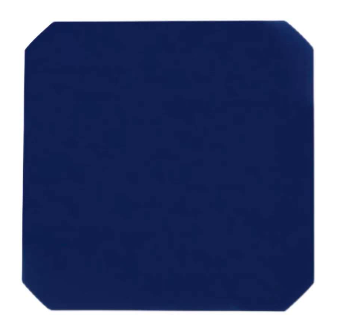
\includegraphics[width=0.36\textwidth]{figures/solar_cell_sunpower_6w.png}
    \caption{SunPower 6W monocrystalline silicon solar cell used as the reference photovoltaic cell for the Solift solar subsystem.}
    \label{fig:solar-cell-sunpower}
\end{figure}

The solar experiment was set up to obtain the I-V and P-V behavior of the cell rather than only one operating point. In an I-V test, the external load is varied from the open-circuit condition to the short-circuit condition. At open circuit, the current is zero and the cell reaches its maximum voltage, \(V_{oc}\). At short circuit, the voltage approaches zero and the current reaches \(I_{sc}\). Between these two ends, the product \(P=VI\) first rises and then falls. The highest point on the P-V curve is the maximum power point, defined by \(V_{mp}\), \(I_{mp}\), and \(P_{mp}\). This point matters more for aircraft design than either \(V_{oc}\) or \(I_{sc}\) alone, because a real electrical system must draw power near the maximum power region if the solar cells are expected to help the battery.

\begin{figure}[htbp]
    \centering
    \begin{minipage}{0.42\textwidth}
        \centering
        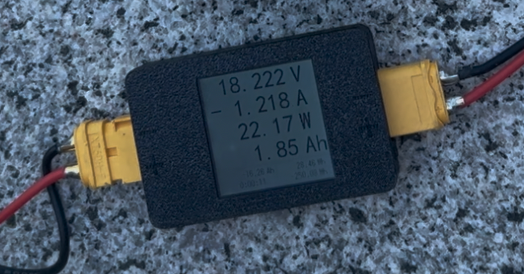
\includegraphics[width=0.95\textwidth]{figures/xt60_meter.png}
        \caption{XT60 inline meter used to read voltage, current, and power during solar cell loading tests.}
        \label{fig:xt60-meter}
    \end{minipage}
    \hfill
    \begin{minipage}{0.42\textwidth}
        \centering
        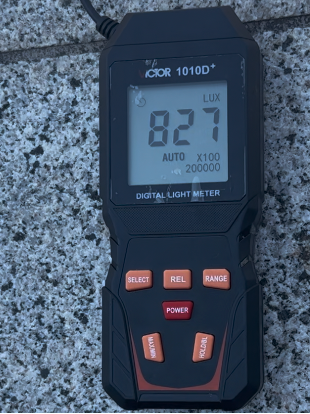
\includegraphics[width=0.75\textwidth]{figures/victor_lux_meter.png}
        \caption{Victor 1010D+ lux meter used to check the illumination level near the tested solar cell.}
        \label{fig:victor-lux-meter}
    \end{minipage}
\end{figure}

The cell was illuminated by a lamp at about \(82{,}000\)-\(84{,}500~\mathrm{lux}\), with the distance between the light source and the cell held near \(160~\mathrm{mm}\). Voltage, current, and power were read using the XT60 inline meter shown in Figure~\ref{fig:xt60-meter}, and illumination was checked with the Victor 1010D+ lux meter shown in Figure~\ref{fig:victor-lux-meter}. The test was conducted at room temperature, approximately \(20\)-\(25^\circ\mathrm{C}\). The report material estimates the combined uncertainty from the lux meter, voltage measurement, current measurement, and resistor tolerance at roughly 5-10\% for the calculated power. That uncertainty is acceptable for feasibility analysis. It is not tight enough for final product certification, but it is good enough to tell whether the solar cells are only decorative or whether they can supply a meaningful amount of electrical power.

In the single-cell test, the measured open-circuit voltage was approximately \(V_{oc}=0.653~\mathrm{V}\), and the short-circuit current was approximately \(I_{sc}=8.813~\mathrm{A}\). The maximum power point occurred near \(V_{mp}=0.480~\mathrm{V}\) and \(I_{mp}=8.096~\mathrm{A}\), giving \(P_{mp}=3.886~\mathrm{W}\). The corresponding fill factor was approximately 0.675. This fill factor is lower than what would be expected from an idealized cell, but it is believable for a practical test setup because series resistance, contact resistance, lamp spectrum, cell temperature, and measurement uncertainty all affect the curve. For the 18-cell series string, the ideal open-circuit voltage scales as \(18 \times 0.653 \approx 11.75~\mathrm{V}\), while the current remains close to the current of one cell if the cells are similarly illuminated. The actual 18-cell string delivered a measured maximum power of \(65.48~\mathrm{W}\) at \(11.462~\mathrm{V}\) and \(5.713~\mathrm{A}\). This result is close enough to the theoretical value of \(18 \times 3.886 \approx 69.95~\mathrm{W}\) to support the solar subsystem as a useful auxiliary source. It should still be described carefully. The solar array can help the aircraft during cruise, testing, and ground exposure under light, but it cannot replace the main battery during high-power vertical takeoff.

The technical feasibility of the wing is supported by the adopted geometric and aerodynamic choices from the same design material. The project uses a stacked triplane arrangement with straight rectangular planforms. Each wing has a span of \(1200~\mathrm{mm}\) and a chord of \(480~\mathrm{mm}\), giving an area of \(0.576~\mathrm{m^2}\) per wing and an aspect ratio of 2.5. The selected airfoil is MH114. This configuration is not the most aerodynamically efficient possible layout, but it is reasonable for the project because it gives the aircraft a large lifting area without forcing the team to manufacture and transport a very long single wing. The rectangular planform also keeps the rib templates, foam cutting process, spar layout, and covering operation much simpler than a tapered planform would. In a course project, that manufacturing simplicity is not a small detail. It is one of the reasons the wing can be built with enough repeatability to make the rest of the design meaningful.

The proposed wing structure is also feasible for a student manufacturing environment. The internal balsa framework provides the main load path through spars, ribs, and local reinforcements. The XPS foam shell helps preserve the airfoil contour and increases local stiffness. The outer heat-shrink film improves surface smoothness and protects the foam and wood structure. This combination is not as strong as a fully molded carbon-fiber wing, but it is easier to fabricate with accessible tools. It also allows the team to repair or adjust the structure without expensive tooling. For a DFM project, this is an important advantage because the manufacturing process can be described step by step and connected to the final aircraft performance.

The claw or fixture is feasible because it can be produced using common student-level manufacturing processes such as 3D printing, laser cutting, or CNC machining, depending on the final material choice. The CAD images show a fixture-like structure with screw holes, arms, and local mounting features. Its job is not only to hold a payload but also to transfer load into the fuselage without creating large local deformation. The design must leave enough space for assembly tools, wiring, and inspection. It must also avoid unnecessary mass, because any mass added to the fixture reduces useful payload or endurance. The current CAD model appears feasible because it uses a simple plate-and-arm geometry rather than a closed shape that would be difficult to access during assembly.

The foldable propeller is feasible as a purchased or modeled subsystem, but it introduces more manufacturing sensitivity than a fixed propeller. A fixed propeller has fewer moving parts and is easier to balance. A foldable propeller adds hinge pins, blade roots, stops, and local clearances. These features allow the blades to fold during storage or after shutdown, but they must deploy symmetrically during operation. If one blade has more friction than the other, deployment can be delayed or uneven. If the hinge clearance is too large, the propeller can vibrate. If the clearance is too small, the blade may bind. This makes the foldable propeller a useful DFM topic because it is simple in appearance but sensitive in operation.

The tilt-rotor mechanism is the most demanding subsystem from a technical feasibility point of view. A fixed motor mount only needs to hold the motor at one angle. A tilt mount must rotate between two functional positions while maintaining stiffness, alignment, and repeatability. During vertical takeoff, the rotor thrust acts mainly upward. During cruise, the same propulsion unit must produce forward thrust. During transition, the loads and moments change continuously. The mechanism therefore needs a clear rotation axis, a controlled bearing or hinge support, a reliable actuator connection, and some way of limiting or locking the end positions. The CAD and video material show that the project has already considered this mechanism, but physical validation would still be needed before flight.

The economic feasibility of Solift is acceptable because the design avoids manufacturing methods that would be unrealistic for the project scale. The solar cells can be purchased as commercial cells. The wing can be built from balsa, XPS foam, adhesive, and covering film. The fixture can be printed or machined. The foldable propeller can be selected from existing UAV propeller designs or manufactured as a small mechanical assembly for demonstration. The tilt mechanism may require the highest precision, but even there the first prototype can use a simplified actuator mount and standard bearings or shafts. This approach keeps the project within a student budget while still allowing meaningful engineering analysis.

The schedule feasibility is also reasonable if the team treats the aircraft as a set of parallel subsystems. The solar testing can be conducted independently of the wing fabrication. The wing airfoil templates and foam shell can be prepared while the fixture is modeled. The foldable propeller can be evaluated separately before it is integrated with the motor. The tilt mechanism can be designed and checked in CAD before the final propulsion installation. This division does not remove the need for final integration, but it prevents the project from depending on a single long manufacturing chain. In a course timeline, that matters. Subsystems that can be developed in parallel give the team more opportunities to recover if one part needs redesign.

Operationally, Solift is feasible as a concept because each subsystem contributes to a recognizable mission sequence. Before operation, the foldable propeller reduces the risk of blade damage during storage and transport. During takeoff, the tilt-rotor mechanism provides vertical lift. During cruise, the wing supplies most of the lift, reducing the power demand compared with a pure multirotor. During daylight operation, the solar cells can reduce net battery draw. During delivery, the claw or fixture holds the payload in a controlled position. During landing and post-flight handling, the compact propulsion arrangement again helps protect the aircraft. The feasibility analysis therefore supports continuing with Solift as the selected object, while also identifying the tilt mechanism and folding propeller as the subsystems that require the most careful validation.

\section{Phase 2: Conceptual design}
\label{subsec:phase2-conceptual}

The conceptual design phase defines how the major subsystems of Solift work together before the detailed geometry is fixed. At this stage, the aircraft is considered as an integrated system rather than as a set of isolated parts. The solar cells, wing, fixture, foldable propeller, and tilt-rotor mechanism each have a separate function, but none of them can be designed properly without considering the others. The solar cells need wing area and a smooth surface. The wing must keep its airfoil shape while carrying the solar cells and internal structure. The fixture must hold the payload without moving the center of gravity too far from the intended range. The propeller must provide thrust while also folding safely during non-operating conditions. The tilt mechanism must rotate the propulsion unit without creating excessive play or misalignment.

The high-level aircraft architecture uses the wing as both an aerodynamic surface and an energy-collection platform. This dual role creates one of the central design problems. A wing normally benefits from a smooth, continuous surface with controlled curvature. A solar cell, however, is a fragile electrical component that must be bonded, wired, and protected. If the solar cells are mounted poorly, they can create surface steps, wiring bumps, or local stiffness changes. These defects may reduce aerodynamic quality and may also create stress concentrations in the cell or adhesive layer. The conceptual design therefore treats the solar layout and the wing structure as one combined design problem rather than two separate tasks.

The payload fixture is placed near the fuselage or central body region because this location reduces the effect of payload mass on pitching moment. A payload mounted too far forward or too far aft would require larger trim corrections and could reduce stability. A payload mounted too far below the aircraft would also increase the moment during acceleration and landing. The fixture therefore has to be compact, stiff, and accessible. It should allow the payload to be installed and removed without disturbing the solar wiring, wing covering, or propulsion system. The current CAD material shows a fixture and payload bay region that can be developed into this role.

The foldable propeller is included at the conceptual stage because logistics UAVs are handled more often than conventional model aircraft. They may be stored, transported, placed near payload stations, and moved between test areas. A long fixed propeller can be damaged easily during these operations. A foldable propeller reduces that risk and can make the aircraft easier to pack. The trade-off is that the blade root becomes more complex. The design must provide a hinge, a stop, and enough stiffness after deployment. This is acceptable because the added complexity is local and because the foldable mechanism can be inspected and tested as a separate part.

The tilt-rotor mechanism is the main feature that separates Solift from a standard fixed-wing solar UAV. In vertical flight, the rotor must direct thrust downward. In cruise, it must rotate to provide forward thrust. Conceptually, this allows the aircraft to combine VTOL operation with wing-borne efficiency. The mechanism must therefore be treated as a primary load-bearing system. It is not a decorative movement or a convenience feature. If the tilt axis is weak, if the actuator linkage has backlash, or if the end positions are not repeatable, the aircraft may lose thrust alignment during transition. The conceptual design therefore assigns the tilt mechanism a higher manufacturing priority than non-load-bearing fairings or cosmetic surfaces.

Figure~\ref{fig:concept-draft} presents the initial hand-drawn concept sketches produced at the start of Phase~2. The upper sketch explores the tilt-rotor nacelle mechanism, annotating the servo motor axis and the two extreme positions (vertical thrust for hover, horizontal for cruise). The lower sketch establishes the overall aircraft layout, identifying the solar panel wing, dual tilting rotors, and ventral cargo bay — the three defining features carried forward into the detailed CAD model.

\begin{figure}[htbp]
    \centering
    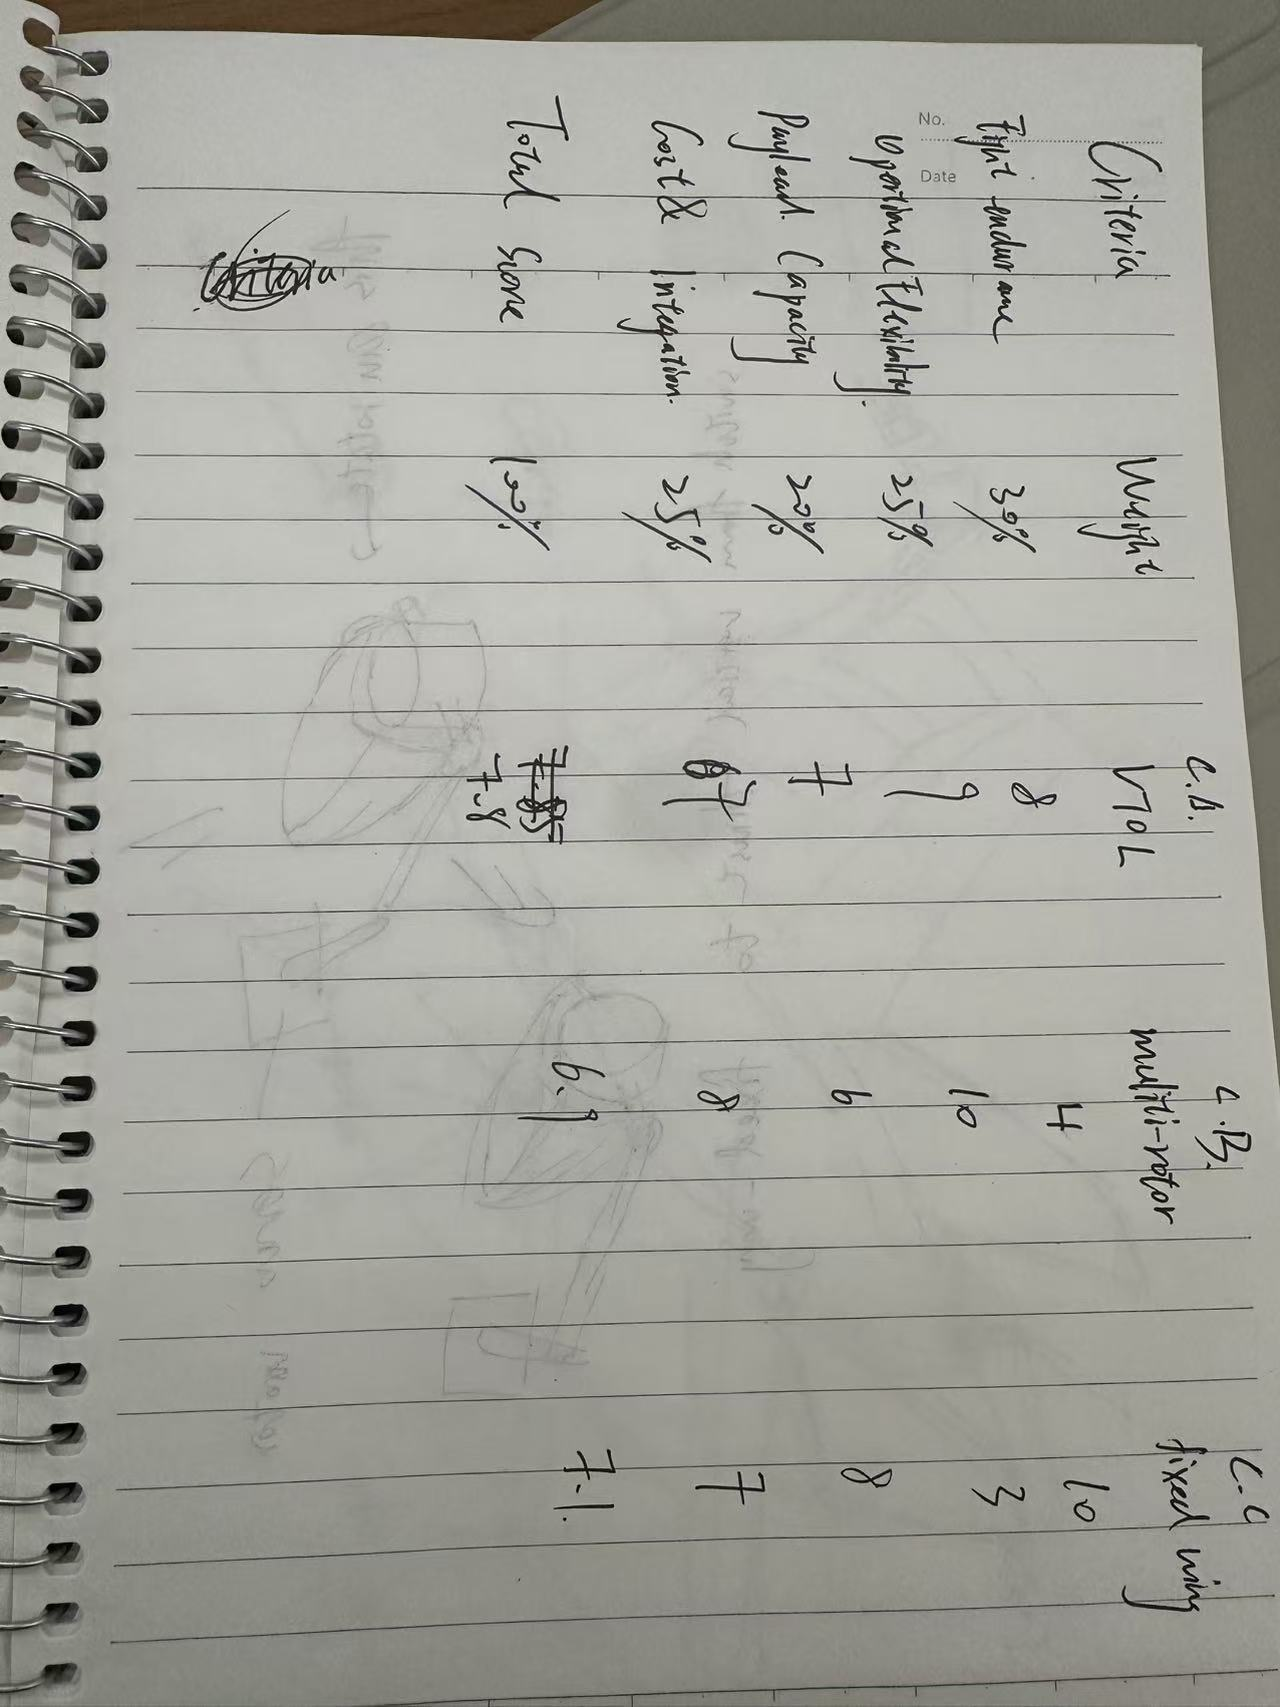
\includegraphics[angle=90,width=0.88\textwidth]{figures/conceptdesign_draft.jpg}
    \caption{Initial concept sketches: tilt-rotor nacelle mechanism (\textit{top}) and overall UAV layout (\textit{bottom}).}
    \label{fig:concept-draft}
\end{figure}

\begin{figure}[htbp]
    \centering
    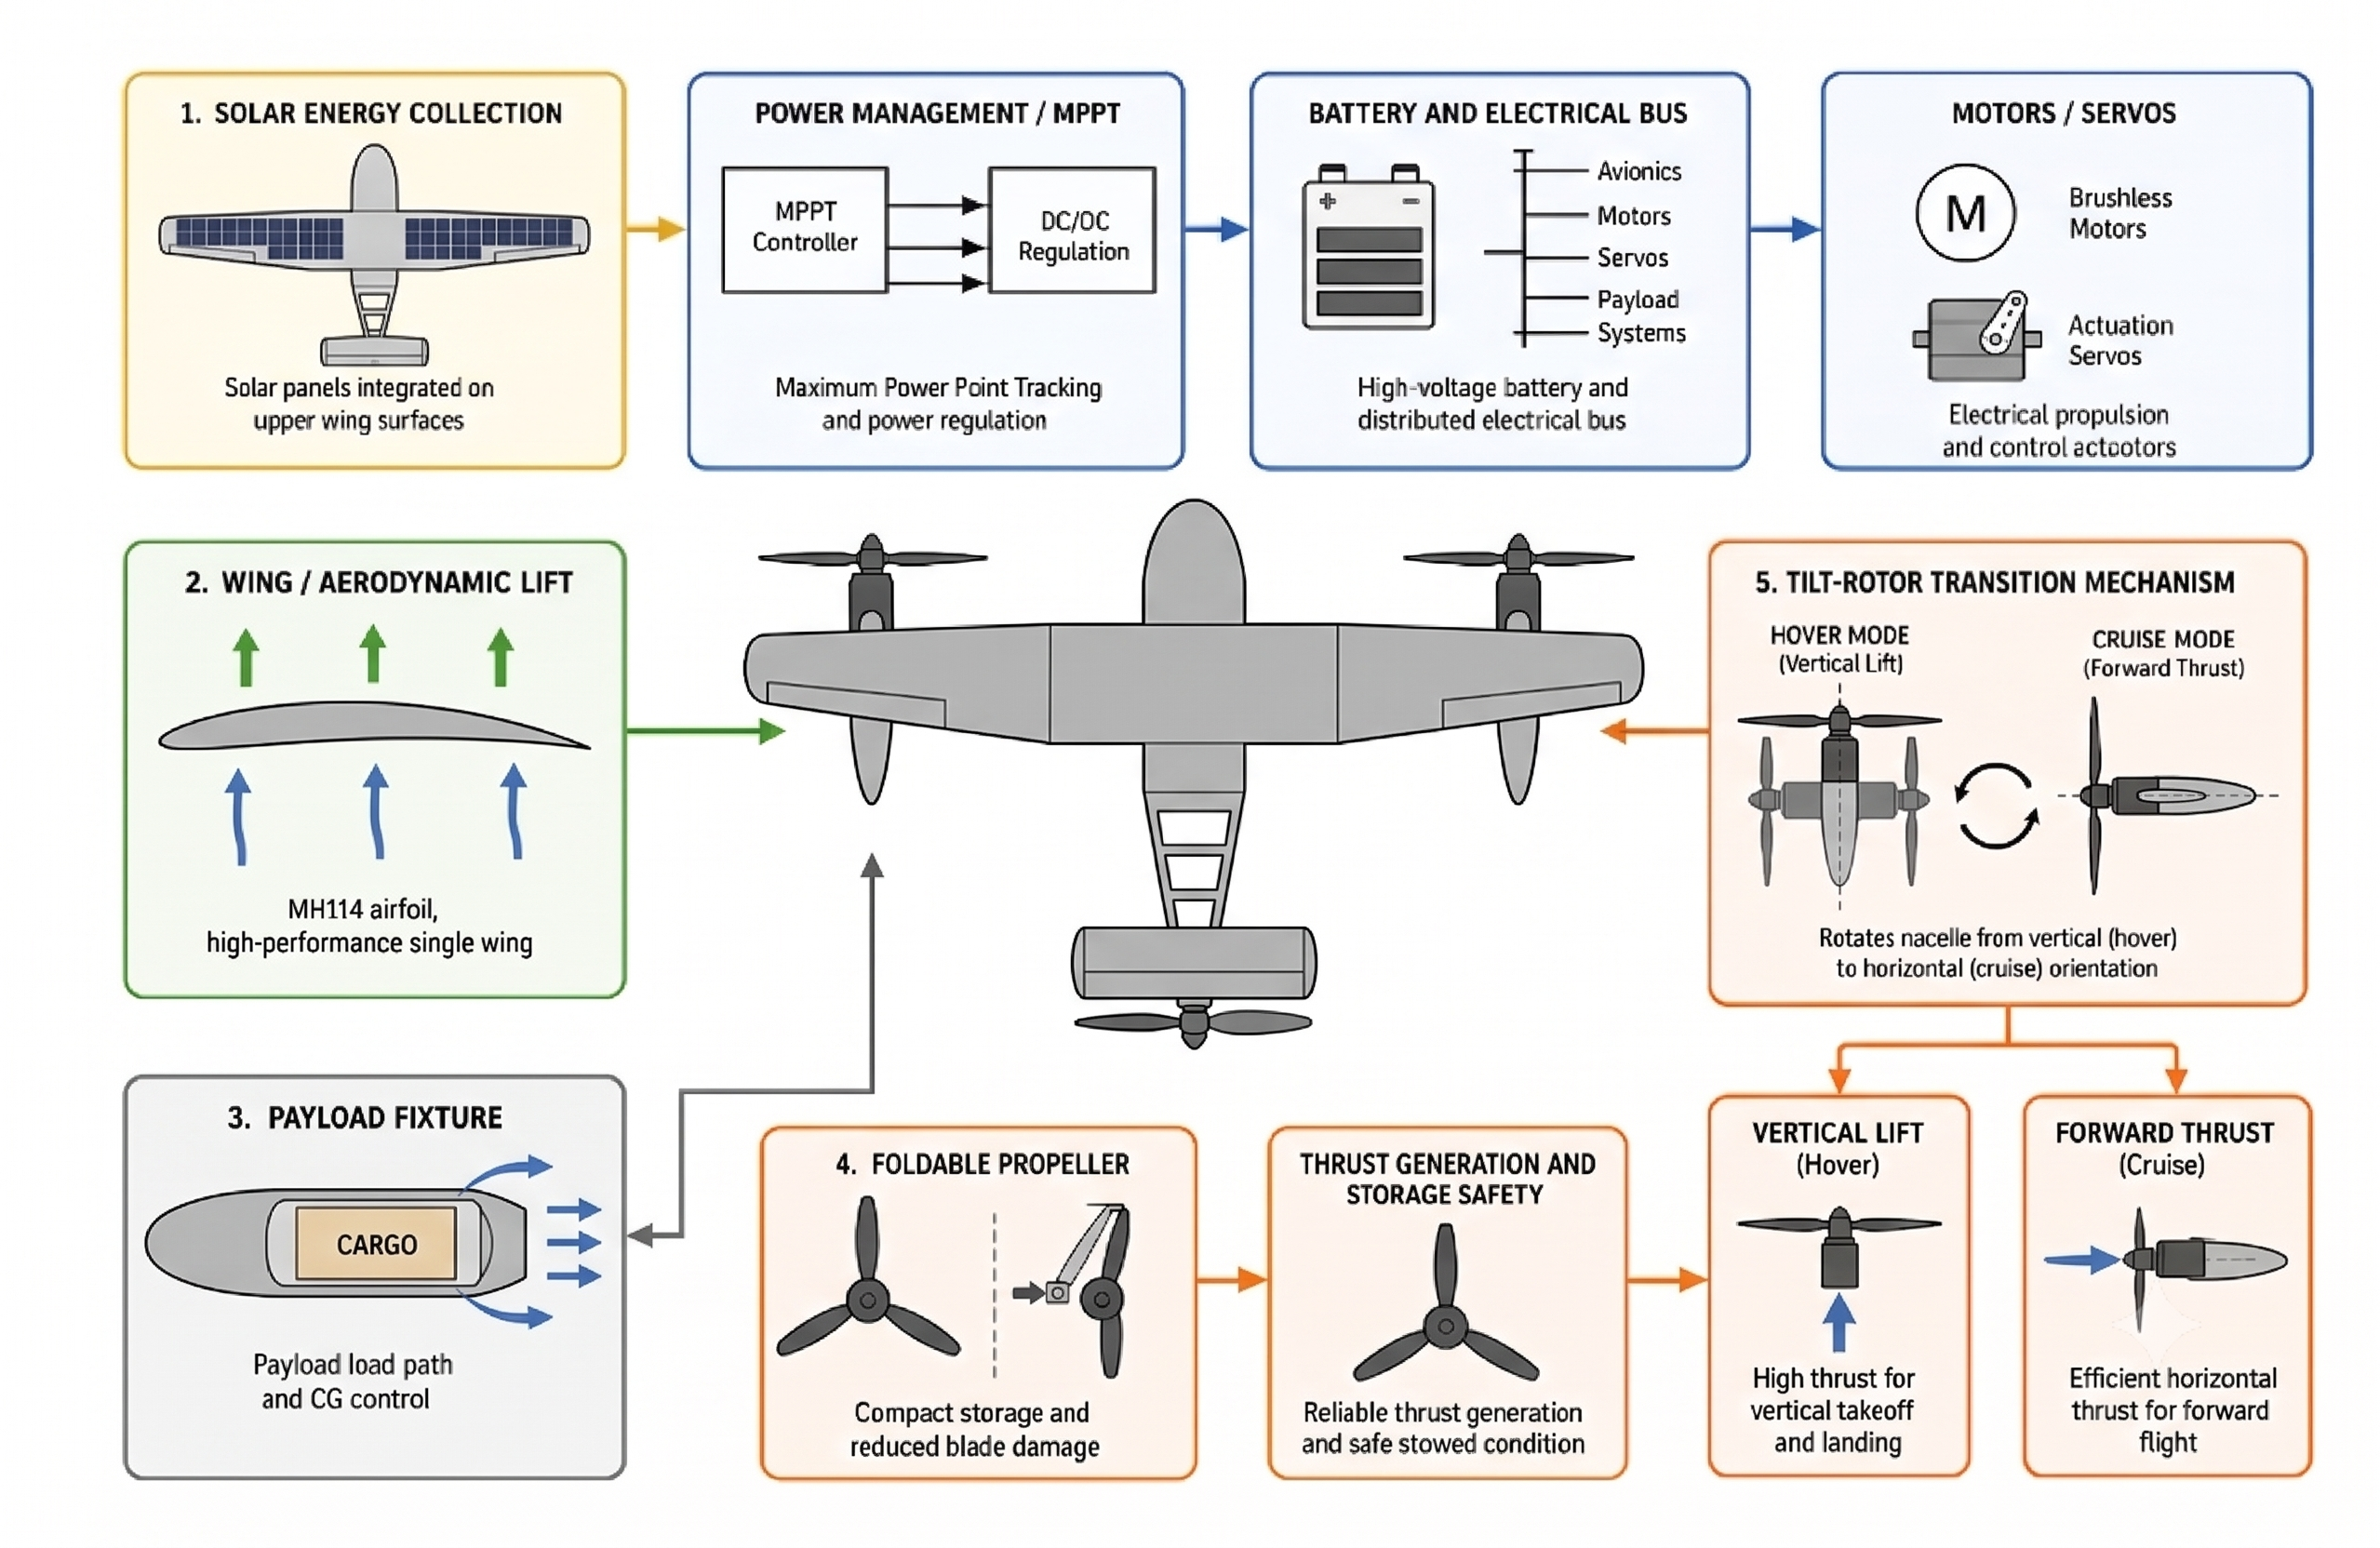
\includegraphics[width=0.9\textwidth]{figures/conceptual_block_diagram.png}
    \caption{Conceptual subsystem architecture of the Solift UAV.}
    \label{fig:conceptual-block-diagram}
\end{figure}

The overall CAD view in Figure~\ref{fig:overall-cad-view} supports the conceptual arrangement. The aircraft body, wing, propulsion components, and rear support structure are visible as one integrated layout. At the conceptual level, this view is useful because it shows that the design is not only a collection of independent parts. The location of each subsystem constrains the others.

\begin{figure}[htbp]
    \centering
    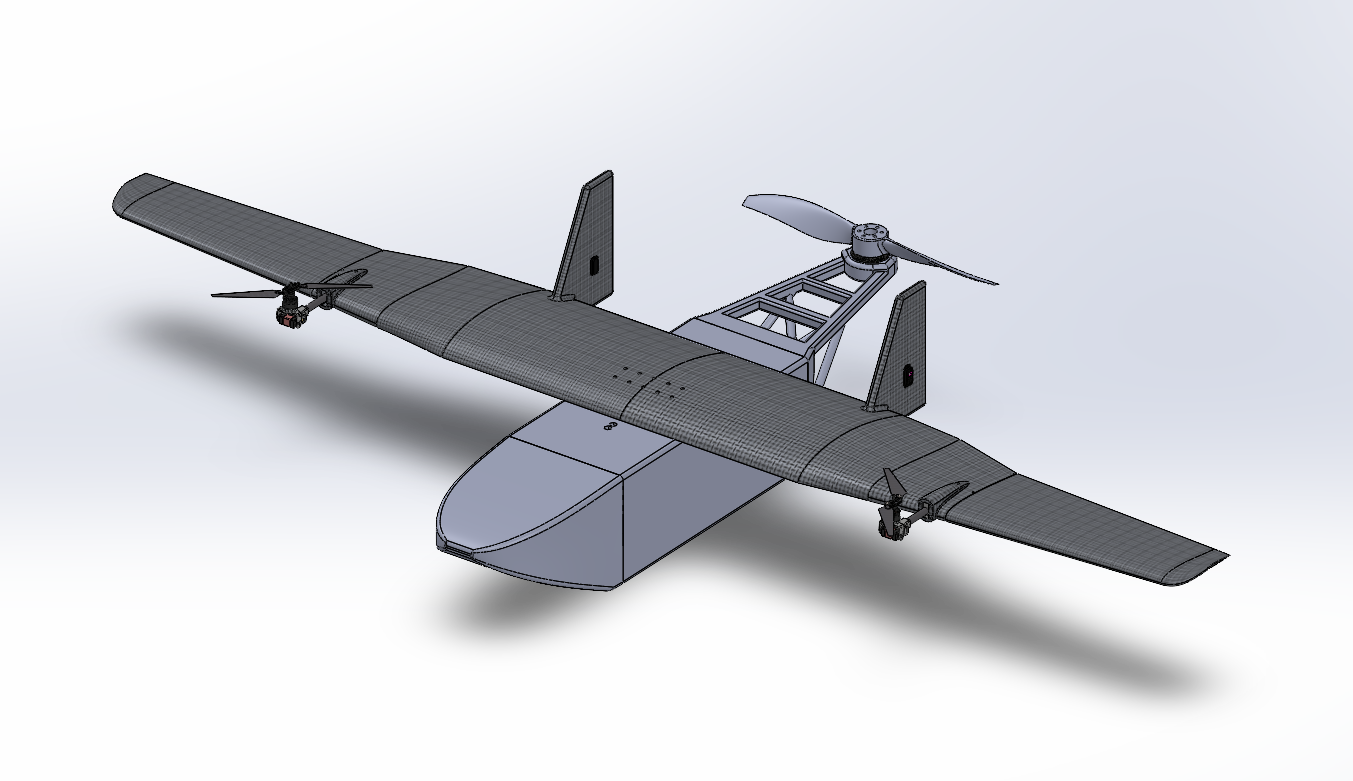
\includegraphics[width=0.88\textwidth]{figures/uav_overall_cad.png}
    \caption{Overall CAD view of the Solift configuration showing the wing, fuselage, propulsion layout, and rear structure.}
    \label{fig:overall-cad-view}
\end{figure}

\begin{figure}[htbp]
    \centering
    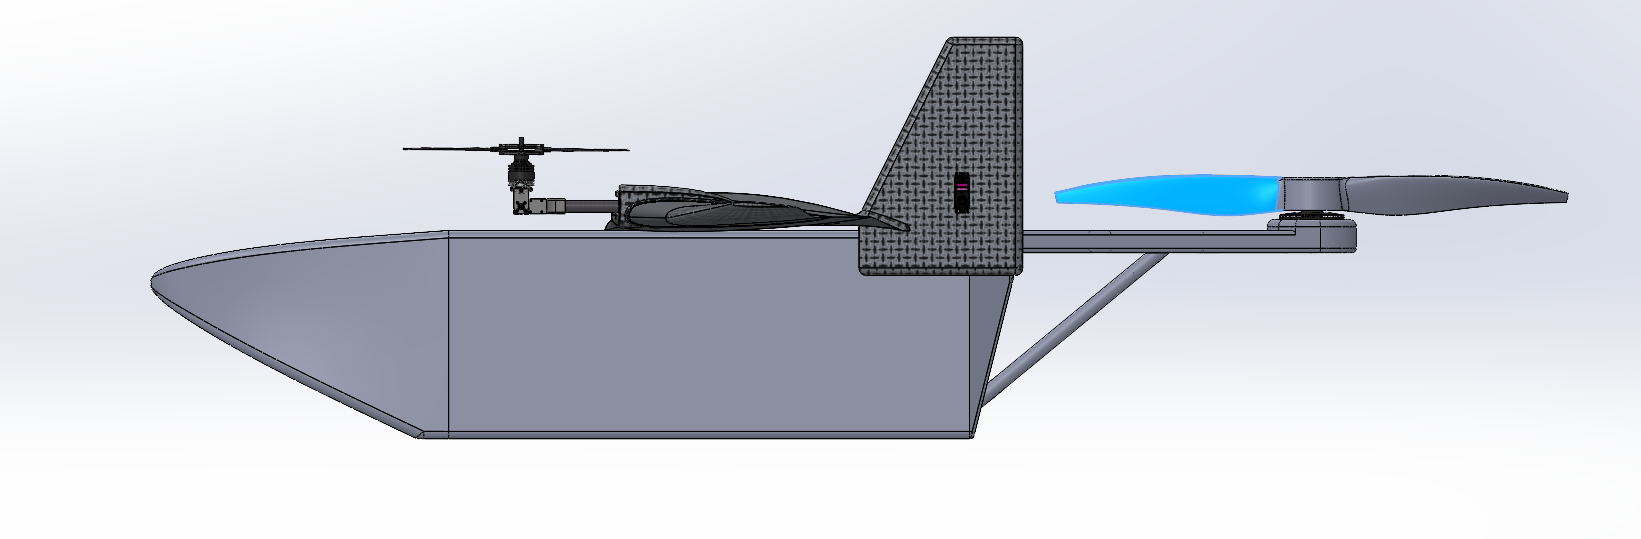
\includegraphics[width=0.88\textwidth]{figures/uav_side_view.png}
    \caption{Side view of the CAD model, useful for checking payload volume, tail arrangement, and propulsion installation height.}
    \label{fig:side-cad-view}
\end{figure}

The conceptual design therefore freezes the main functional layout without pretending that every detail has already been optimized. The aircraft will use solar cells on the lifting surfaces, an MH114-based wing structure, a central fixture or claw for payload handling, foldable propeller hardware for compact handling, and a tilt-rotor mechanism for the transition between vertical and forward flight. The later design phases refine how these functions are physically embodied.

\section{Phase 3: Embodiment design}
\label{subsec:phase3-embodiment}

The embodiment design phase turns the conceptual architecture into physical forms, materials, and approximate manufacturing routes. In this phase, the design is still flexible, but the main geometry and material logic become visible. For Solift, embodiment design is especially important because several subsystems share the same space. The solar cells occupy the wing surface. The wing structure carries aerodynamic loads and supports the cell layout. The payload fixture sits inside or under the fuselage region. The foldable propeller and tilt-rotor mechanism are connected to the propulsion layout. Each subsystem must be manufacturable on its own and compatible with the assembly around it.

The wing embodiment uses a stacked triplane arrangement with rectangular planforms. Each wing has a span of \(1200~\mathrm{mm}\), a chord of \(480~\mathrm{mm}\), and an area of \(0.576~\mathrm{m^2}\). The selected airfoil is MH114, which was chosen for low-speed UAV operation where high lift and gradual stall behavior are more valuable than high-speed efficiency. The aerodynamic-section data in Figure~\ref{fig:mh114-aero-curves} show the basic reason for using this airfoil. The lift coefficient rises to a high value before stall, and the lift-to-drag ratio remains useful over the moderate positive angle-of-attack range expected for a small slow aircraft. The Word report notes that at a representative Reynolds number near \(4 \times 10^5\), the MH114 section can reach a section lift coefficient of about 1.7 at an angle of attack near \(10^\circ\), with a maximum lift coefficient above 1.6 and a stall trend that is gradual rather than abrupt. These values should not be treated as final whole-aircraft performance numbers, because the real triplane arrangement, fuselage, propellers, and manufacturing errors will change the flow. They are still useful at this stage because they justify choosing a high-lift low-speed airfoil instead of a thin high-speed section.

\begin{figure}[htbp]
    \centering
    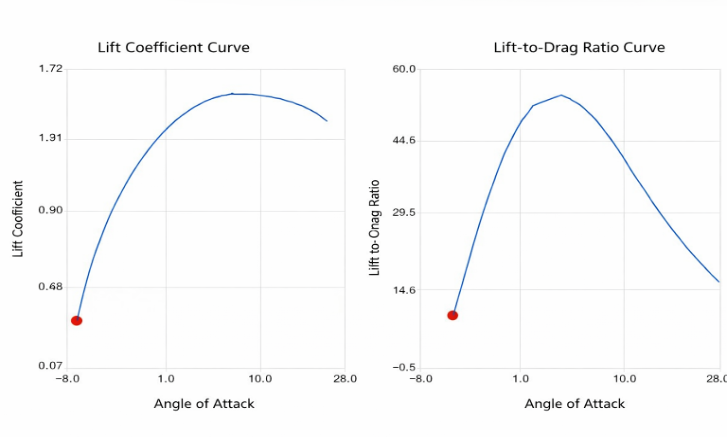
\includegraphics[width=0.78\textwidth]{figures/mh114_aero_curves.png}
    \caption{Adopted MH114 aerodynamic-section data, with lift coefficient curve on the left and lift-to-drag ratio curve on the right.}
    \label{fig:mh114-aero-curves}
\end{figure}

The triplane layout increases total lifting area without requiring a very long single wing. That choice is practical for this project. A single large wing would be cleaner aerodynamically, but it would also need a longer spar, more careful bending stiffness design, and more storage space. It would be easier to damage during transport. The stacked rectangular wings are not as elegant, but they are easier to build, inspect, and repair. The rectangular planform also lets the team repeat ribs and foam templates rather than cutting a different section for every spanwise station. For a student manufacturing project, that repeatability is valuable because a wing that is theoretically better but poorly made is not better in practice.

The embodied wing structure consists of a balsa internal framework, an XPS foam shell, and an outer covering film. The balsa framework forms the skeleton. It carries bending and shear loads through spars, ribs, and local reinforcements. Balsa is light and easy to cut, which makes it suitable for a student prototype, but it must be protected from crushing and moisture. The XPS foam shell surrounds the framework and helps maintain the airfoil contour. This is important because the MH114 section only provides the expected aerodynamic behavior if the manufactured wing remains close to the designed shape. A small dent, uneven covering tension, or poorly aligned foam shell can change the local camber enough to affect lift and drag. The covering film gives the wing a smoother outer surface and adds a small skin effect that ties the structure together. The film also provides a practical surface finish without requiring a molded composite shell.

The solar cells are embodied as surface-mounted photovoltaic elements bonded to the wing or selected upper surfaces. The chosen SunPower cells are efficient, but they are also thin and brittle compared with the wing materials around them. Their installation must therefore avoid forcing the cell into excessive curvature. A flat or gently curved surface is preferred. The adhesive layer should be thin enough to avoid a raised edge but compliant enough to avoid cracking the cell under small wing deflections. The wiring should be routed in channels or low-profile paths so that it does not create bumps on the aerodynamic surface. The wing is already doing two jobs: lifting the aircraft and carrying the energy surface. Because of that, the solar cell cannot be treated as a sticker added after the wing is finished. Its position, wire exit direction, and protection layer have to be planned while the wing structure is still being designed.

The payload fixture is embodied as a CAD-modeled mechanical holder with arms, screw holes, and local support surfaces. Figures~\ref{fig:payload-fixture-installed} and~\ref{fig:payload-fixture-detail} show the fixture region and a separate fixture view. The design uses open geometry rather than a closed box. This is a practical choice because it leaves access for fasteners and inspection. The fixture should transfer load into the fuselage floor or frame through several attachment points rather than through one thin wall. It also needs enough local stiffness to prevent the payload from shifting during takeoff, landing, or transition. In a small UAV, even a small payload shift can change the center of gravity and affect control.

\begin{figure}[htbp]
    \centering
    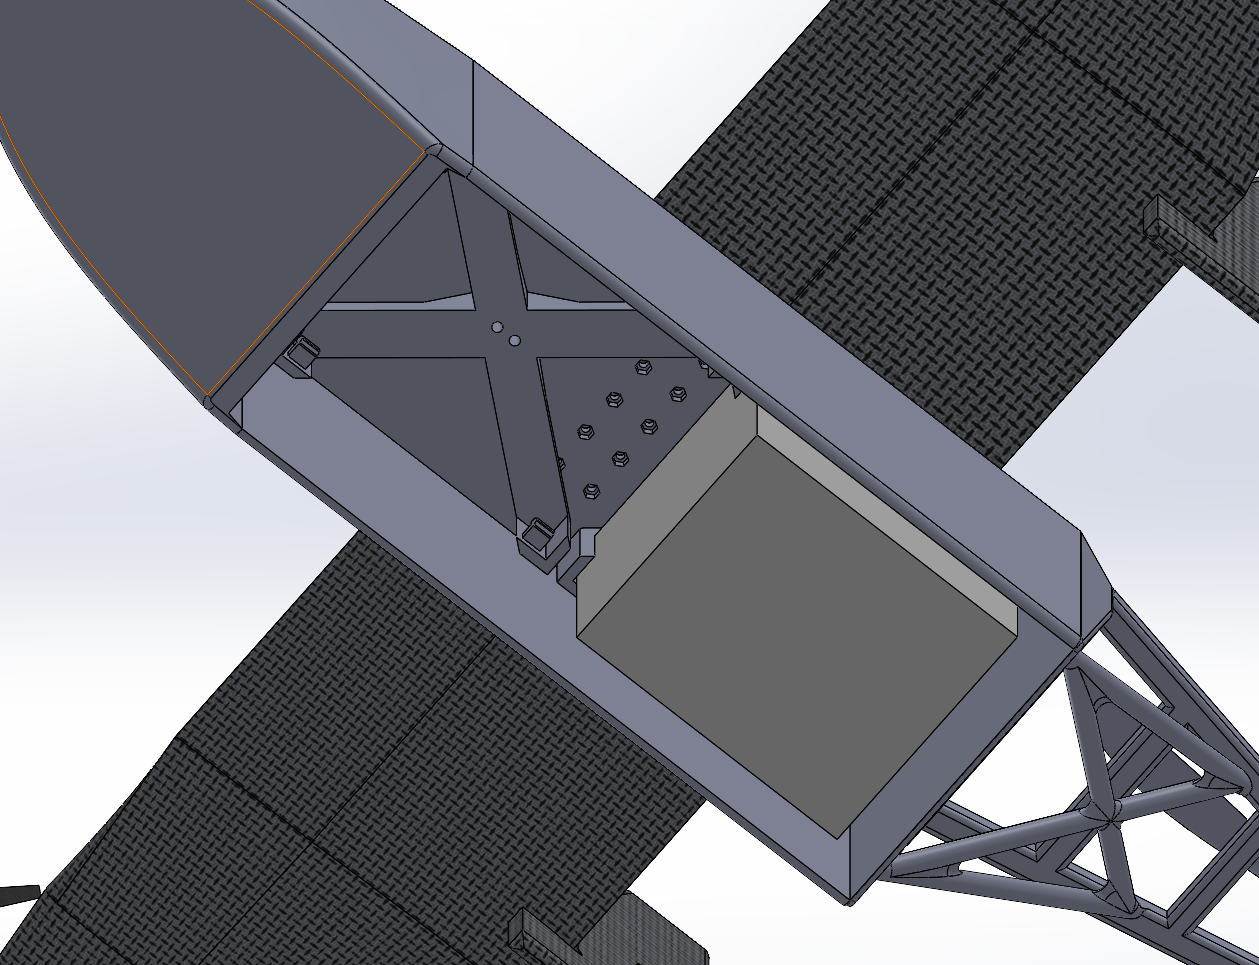
\includegraphics[width=0.82\textwidth]{figures/payload_fixture_installed.png}
    \caption{CAD view of the payload bay and fixture region, showing the mounting area and surrounding fuselage structure.}
    \label{fig:payload-fixture-installed}
\end{figure}

\begin{figure}[htbp]
    \centering
    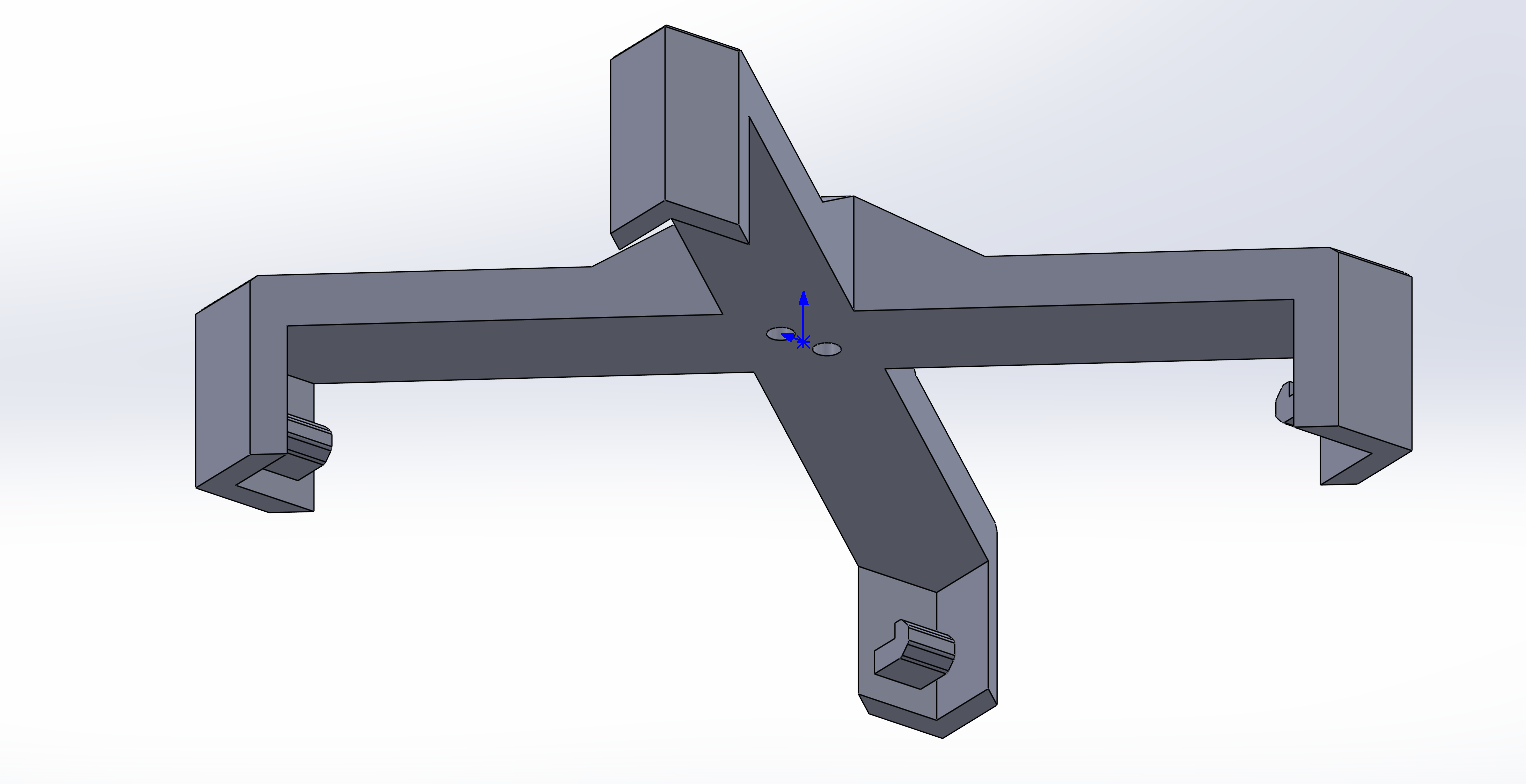
\includegraphics[width=0.78\textwidth]{figures/payload_fixture_detail.png}
    \caption{Standalone fixture geometry with arms and mounting features. The open layout improves access for assembly and inspection.}
    \label{fig:payload-fixture-detail}
\end{figure}

The foldable propeller is embodied as a two-blade assembly with hinged blade roots. The CAD images show the folded and deployed configurations. The blades appear to use a composite or carbon-fiber texture, which is appropriate for a propeller because stiffness-to-mass ratio is important. The hinge and central hub are the critical manufacturing features. A blade that folds neatly in CAD may still fail in practice if the hinge holes are misaligned, if the pin fit is poor, or if the blade root rubs against the hub. The embodied design must therefore provide enough bearing area around the hinge and a clear mechanical stop for the deployed position.

\begin{figure}[htbp]
    \centering
    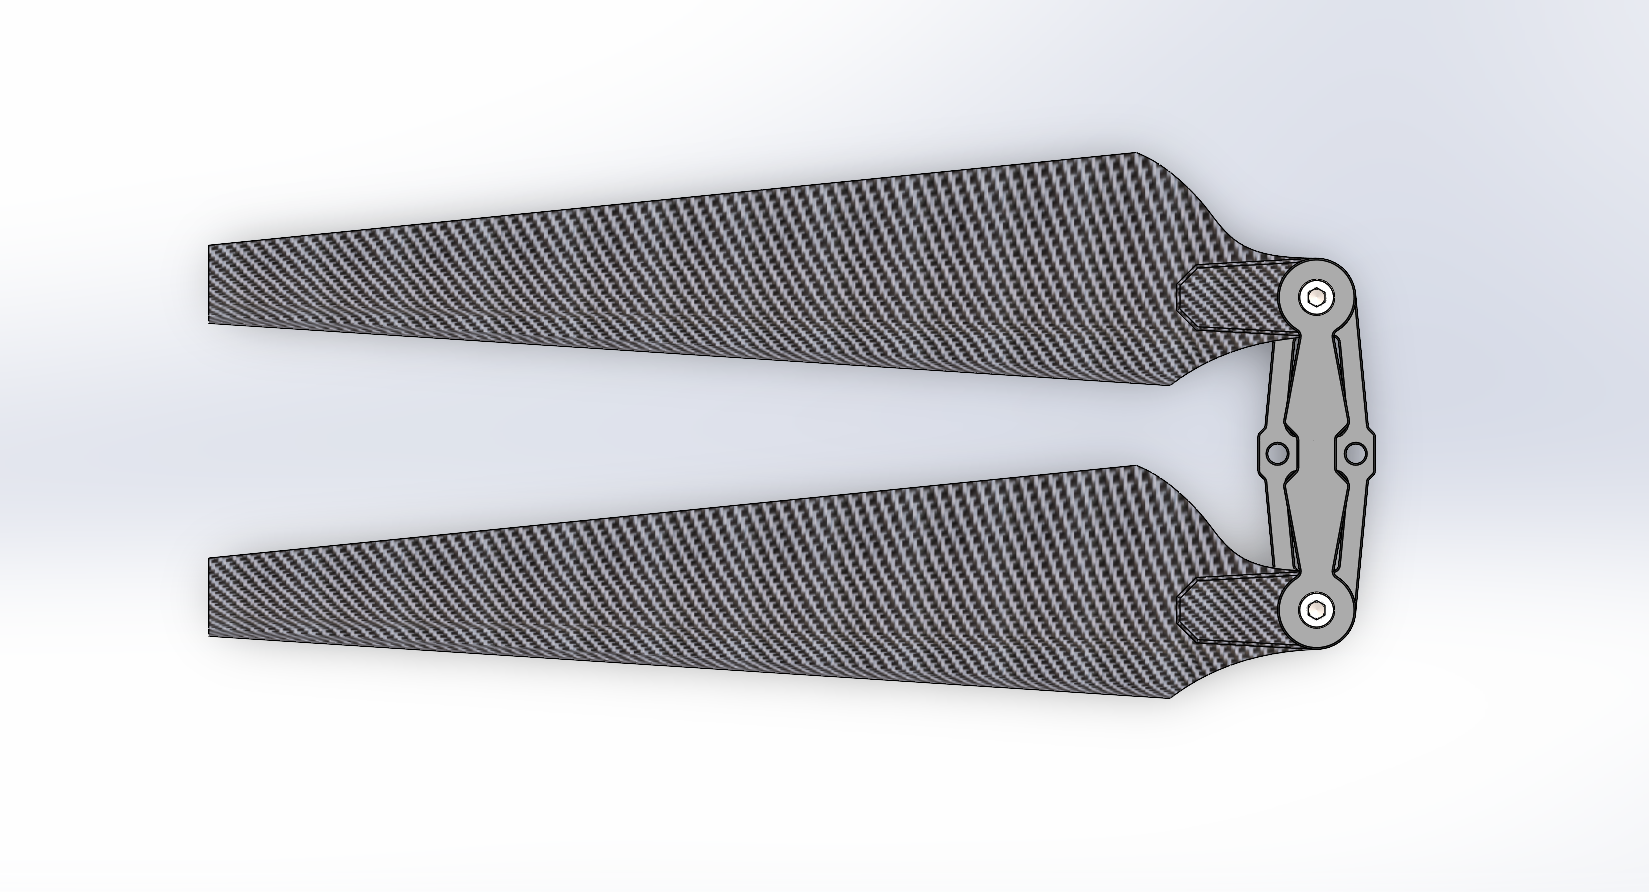
\includegraphics[width=0.78\textwidth]{figures/foldable_propeller_folded.png}
    \caption{Foldable propeller model showing the two blades near the folded storage position.}
    \label{fig:foldable-propeller-folded}
\end{figure}

\begin{figure}[htbp]
    \centering
    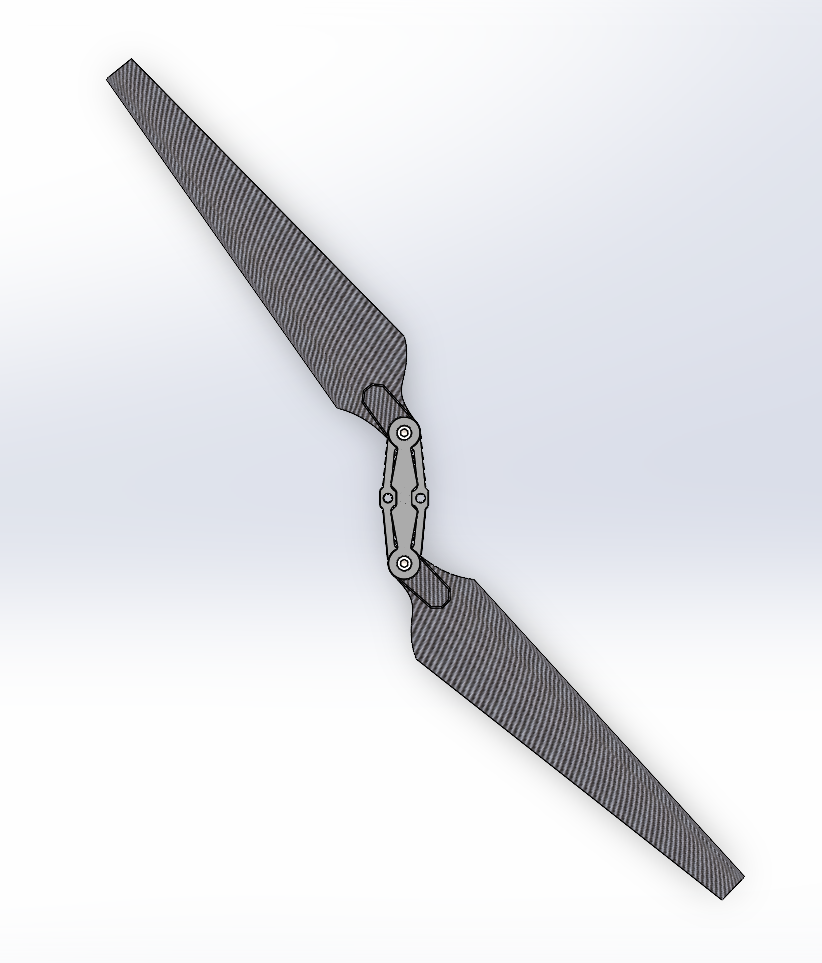
\includegraphics[width=0.58\textwidth]{figures/foldable_propeller_angle.png}
    \caption{Foldable propeller in an intermediate or angled configuration, showing the hinge region and blade-root geometry.}
    \label{fig:foldable-propeller-angle}
\end{figure}

\begin{figure}[htbp]
    \centering
    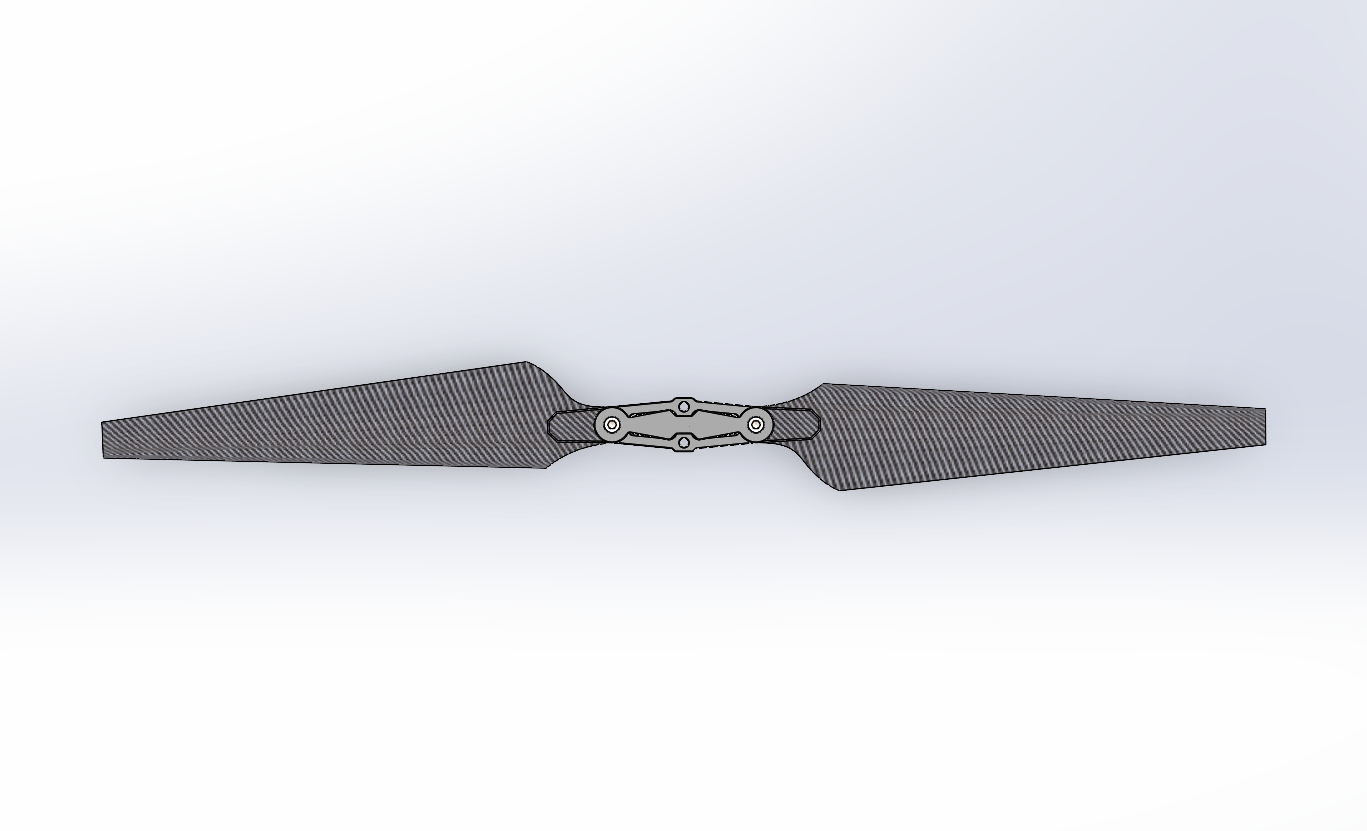
\includegraphics[width=0.78\textwidth]{figures/foldable_propeller_deployed.png}
    \caption{Foldable propeller in deployed configuration. The hub and hinge geometry must hold the blades symmetrically during rotation.}
    \label{fig:foldable-propeller-deployed}
\end{figure}

The tilt-rotor mechanism is embodied as a rotating propulsion support. In the CAD and video material, the motor and propeller are not simply fixed to the wing or tail. They are part of a moving assembly. The embodiment must provide a rotation axis, side support, actuator connection, and end-position control. This mechanism should ideally be compact because large brackets increase drag and mass. It should also be stiff because any angular error changes the thrust direction. A tilt mechanism can look mechanically simple from the outside, but its manufacturing tolerance is more demanding than a static bracket. The shaft, bearing, motor mount, and actuator linkage all affect the final thrust alignment.

The embodiment design choices show that Solift is manufacturable in principle, but they also identify where the design needs care. The wing structure is simple enough to build but sensitive to contour accuracy. The solar cells are available but fragile. The fixture is easy to model but must not become too heavy. The foldable propeller is compact but hinge-sensitive. The tilt mechanism provides the main VTOL function but requires the strictest alignment control. These observations guide the detailed design phase.

\section{Phase 4: Detailed design}
\label{subsec:phase4-detailed}

The detailed design phase records the dimensions, measured values, material decisions, part functions, and manufacturing implications of the selected concept. The purpose is not to claim that the design is already a certified final product. The purpose is to define the design clearly enough that another engineering team could understand what has been chosen, what still needs verification, and which manufacturing issues are most important.

The solar subsystem is summarized first because it is the part of the design with the clearest experimental record. The Word report does not only state that the aircraft uses solar cells; it includes load-test data for a single cell, photographs of the measurement tools, curve plots, and a separate measurement of an 18-cell series string. This matters for DFM because the solar surface is both an electrical subsystem and a manufactured surface. The team has to decide how many cells can fit, how they will be bonded, where the wires will leave the wing, and whether the measured power is large enough to justify the extra manufacturing effort.

Table~\ref{tab:single-cell-raw-data} gives the measured voltage, current, and power points for the single-cell test. The data follow the expected shape. Near open circuit, the voltage is high and the current is zero. As the load decreases, current rises while voltage falls. The power reaches its maximum at an intermediate point, not at either end of the curve. That point, \(0.480~\mathrm{V}\) and \(8.096~\mathrm{A}\), is the most useful operating point from a design perspective because it gives the largest measured power, \(3.886~\mathrm{W}\), under the test condition.

\begin{table}[htbp]
    \centering
    \caption{Measured voltage, current, and power of a single SunPower photovoltaic cell}
    \label{tab:single-cell-raw-data}
    \begin{tabular}{ccc}
        \toprule
        Voltage \(V\) (\(\mathrm{V}\)) & Current \(I\) (\(\mathrm{A}\)) & Power \(P\) (\(\mathrm{W}\)) \\
        \midrule
        0.653 & 0.000 & 0.000 \\
        0.624 & 1.832 & 1.143 \\
        0.613 & 2.246 & 1.377 \\
        0.612 & 2.365 & 1.447 \\
        0.611 & 2.642 & 1.614 \\
        0.604 & 2.873 & 1.735 \\
        0.567 & 4.750 & 2.693 \\
        0.480 & 8.096 & 3.886 \\
        0.067 & 8.813 & 0.590 \\
        \bottomrule
    \end{tabular}
\end{table}

\begin{figure}[htbp]
    \centering
    \begin{minipage}{0.46\textwidth}
        \centering
        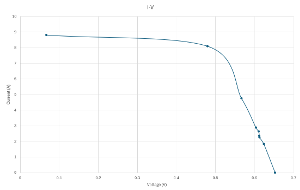
\includegraphics[width=0.96\textwidth]{figures/iv_curve.png}
        \caption{Measured current-voltage curve for the tested solar cell.}
        \label{fig:iv-curve}
    \end{minipage}
    \hfill
    \begin{minipage}{0.46\textwidth}
        \centering
        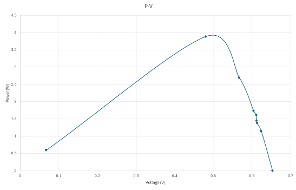
\includegraphics[width=0.96\textwidth]{figures/pv_curve.png}
        \caption{Measured power-voltage curve showing the maximum power point near \(0.480~\mathrm{V}\).}
        \label{fig:pv-curve}
    \end{minipage}
\end{figure}

Figures~\ref{fig:iv-curve} and~\ref{fig:pv-curve} make the same result easier to interpret. The I-V curve drops sharply only near the short-circuit end, while the P-V curve rises to a peak and then falls. For the aircraft, this means the electrical system should not simply connect the cells to a load at an arbitrary voltage. A maximum power point tracking circuit or at least a carefully chosen operating voltage would be needed if the team wants the solar array to produce power close to the measured peak. Without that, the cells could still generate voltage but operate away from their best power region.

The measured values from the single cell and the 18-cell series string are summarized in Table~\ref{tab:solar-measured-data}. These values are used as design inputs for the report. The single-cell result is useful because it shows the behavior of one cell under the test illumination. The 18-cell string result is more relevant to the aircraft because the actual vehicle would need a higher voltage than one cell can provide.

\begin{table}[htbp]
    \centering
    \caption{Measured solar cell and 18-cell string performance used for design}
    \label{tab:solar-measured-data}
    \begin{tabular}{p{0.26\textwidth} p{0.22\textwidth} p{0.40\textwidth}}
        \toprule
        Parameter & Measured value & Design meaning \\
        \midrule
        Cell type &
        SunPower monocrystalline silicon &
        High-efficiency commercial cell suitable for lightweight aircraft surfaces. \\
        Cell side length &
        \(161.7~\mathrm{mm}\) &
        Determines packing layout and available mounting area on the wing. \\
        Rated cell power &
        \(6~\mathrm{W}\) &
        Manufacturer rating; practical output depends on illumination and temperature. \\
        Cell efficiency &
        About \(23.2\%\) &
        Supports the use of limited wing area for energy harvesting. \\
        Single-cell \(V_{oc}\) &
        \(0.653~\mathrm{V}\) &
        Maximum no-load voltage measured in the single-cell test. \\
        Single-cell \(I_{sc}\) &
        \(8.813~\mathrm{A}\) &
        Maximum short-circuit current under the test illumination. \\
        Single-cell \(P_{mp}\) &
        \(3.886~\mathrm{W}\) &
        Practical maximum power point under the test condition. \\
        Fill factor &
        \(0.675\) &
        Indicates real losses from resistance, contacts, illumination, and measurement conditions. \\
        18-cell string maximum power &
        \(65.48~\mathrm{W}\) at \(11.462~\mathrm{V}\), \(5.713~\mathrm{A}\) &
        Confirms that a series string can provide useful auxiliary power for the UAV electrical system. \\
        \bottomrule
    \end{tabular}
\end{table}

For a series string, the voltage ideally adds while the current remains close to the current of one cell. Using the measured single-cell value, the ideal open-circuit voltage of 18 cells is
\[
    V_{oc,total} \approx 18 \times 0.653 = 11.754~\mathrm{V}.
\]
The ideal maximum-power voltage is similarly estimated as
\[
    V_{mp,total} \approx 18 \times 0.480 = 8.64~\mathrm{V},
\]
and the ideal maximum power is approximately
\[
    P_{mp,total} \approx 18 \times 3.886 = 69.948~\mathrm{W}.
\]
The measured 18-cell string delivered \(65.48~\mathrm{W}\) at \(11.462~\mathrm{V}\) and \(5.713~\mathrm{A}\), as shown in the test setup in Figure~\ref{fig:series-18-cell-setup}. The measured maximum is lower than the ideal scaled value, which is expected. Cells in a string are never perfectly matched, the lamp illumination is not perfectly uniform, solder joints add resistance, and the operating point found by fixed loads may not land exactly on the true maximum power point. The result is still close enough to justify the array as a meaningful auxiliary power source. It is not enough to replace the main battery during high-power vertical flight, but it can reduce net energy draw during lower-power phases and can support charging or endurance extension under suitable light.

\begin{figure}[htbp]
    \centering
    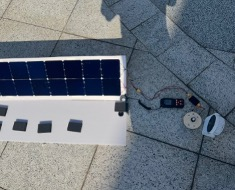
\includegraphics[width=0.48\textwidth]{figures/series_18_cell_setup.jpg}
    \caption{Overall measuring system for the 18-cell series photovoltaic string.}
    \label{fig:series-18-cell-setup}
\end{figure}


The solar cell installation requires more than choosing the number of cells. The cells need a bonding method that keeps them attached without cracking them. A rigid adhesive layer may transmit too much wing strain into the cell. A very soft adhesive may allow local movement and edge peeling. A thick adhesive layer can create a step in the wing surface. The preliminary design therefore favors a thin, uniform bonding layer on a surface region with limited curvature. Wiring should leave the cell through planned channels or low-profile routing paths. If the wiring is placed directly on top of the wing surface, it may disturb the boundary layer and make the covering film difficult to apply. If the wiring is buried too deeply, repair becomes difficult. A practical design should route wires near ribs or spars where possible, because those locations already have structural discontinuities and easier access.

The wing geometry is summarized in Table~\ref{tab:wing-geometry}. The rectangular planform is not the most refined aerodynamic shape, but it is appropriate for this stage because it simplifies manufacturing. A rectangular wing allows repeated ribs, easier foam cutting, and simpler covering. The selected MH114 airfoil gives the project a defined aerodynamic section, so the manufacturing process must aim to preserve that shape. The most important wing manufacturing risk is not the nominal planform dimension; it is contour error. If the foam shell is cut inaccurately or the covering film shrinks unevenly, the actual airfoil can differ from the intended MH114 profile.

\begin{table}[htbp]
    \centering
    \caption{Adopted wing geometry for the Solift concept}
    \label{tab:wing-geometry}
    \begin{tabular}{p{0.34\textwidth} p{0.24\textwidth} p{0.30\textwidth}}
        \toprule
        Parameter & Value & Note \\
        \midrule
        Wing arrangement &
        Stacked triplane &
        Increases lifting area within compact span. \\
        Planform type &
        Straight rectangular wing &
        Simplifies rib, spar, and foam-shell manufacturing. \\
        Span of each wing &
        \(1200~\mathrm{mm}\) &
        Compact enough for student fabrication and handling. \\
        Chord of each wing &
        \(480~\mathrm{mm}\) &
        Provides space for structure and possible solar cell placement. \\
        Area of each wing &
        \(0.576~\mathrm{m^2}\) &
        Calculated from span and chord. \\
        Aspect ratio &
        2.5 &
        Low to moderate value, acceptable for compact low-speed configuration. \\
        Adopted airfoil &
        MH114 &
        Selected for low-speed lift capability and gradual stall behavior. \\
        \bottomrule
    \end{tabular}
\end{table}

The Reynolds-number range also supports the choice of MH114. Using the actual chord length of \(0.480~\mathrm{m}\), a representative low-speed flight range of \(8\)-\(15~\mathrm{m/s}\), and an air kinematic viscosity of about \(1.5 \times 10^{-5}~\mathrm{m^2/s}\), the Reynolds number can be estimated as
\[
    Re = \frac{Vc}{\nu}.
\]
At \(8~\mathrm{m/s}\), this gives \(Re \approx 2.56 \times 10^5\). At \(15~\mathrm{m/s}\), it gives \(Re \approx 4.80 \times 10^5\). This is the low-to-moderate Reynolds-number regime expected for small UAV wings. It is also the regime where surface quality and airfoil fidelity matter. A full-size aircraft wing can sometimes tolerate small local surface errors without a large percentage change in performance. A small UAV wing operating at this Reynolds number has less margin. Rough covering seams, dents in the foam shell, and local steps around solar cells can affect transition, separation behavior, and drag.

The Word report describes the MH114 section as having high lift capability, a maximum lift coefficient above 1.6, and a relatively smooth stall trend. In practical terms, that means the airfoil is forgiving enough for a student-built aircraft but still sensitive enough that poor manufacturing would waste the benefit of the selected section. The design therefore links aerodynamics and manufacturing directly. Choosing MH114 is only half of the decision. The team must also make the wing in a way that keeps the MH114 shape recognizable after foam cutting, framework bonding, film shrinking, and solar cell installation.

The detailed wing structure uses three functional layers. The balsa framework is the main internal load path. The XPS foam shell defines the airfoil surface and supports the covering. The heat-shrink film improves smoothness and ties the surface together. The manufacturing sequence should start with airfoil templates for the foam shell, because the shell sets the external geometry. The internal balsa spars and ribs should be dry-fitted before bonding so that twist can be checked. After the framework is bonded into the shell, the assembly should be inspected from the root and tip to confirm that the chord lines remain consistent. The covering film should then be applied symmetrically and with controlled heat. Too much heat or uneven pulling can warp the wing, especially because the balsa and foam structure is light. These are simple shop operations, but they strongly affect aerodynamic quality.

The solar cells complicate this wing manufacturing sequence. If the cells are bonded before the covering is stabilized, the wing may shift slightly afterward and stress the cells. If the cells are bonded after all covering is complete, the adhesive and wiring can create a raised edge on the aerodynamic surface. The cleaner approach is to reserve defined solar mounting zones on the upper surface, finish the surrounding wing surface, and then bond the cells using a thin controlled adhesive layer. The wire exits should be placed near ribs or planned channels rather than across unsupported foam. This arrangement keeps the electrical assembly accessible while reducing unnecessary surface disturbance.

\begin{table}[htbp]
    \centering
    \caption{Subsystem materials and functions in the detailed concept}
    \label{tab:subsystem-materials}
    \begin{tabular}{p{0.22\textwidth} p{0.26\textwidth} p{0.40\textwidth}}
        \toprule
        Subsystem or part & Preliminary material or component & Function and DFM concern \\
        \midrule
        Solar cell &
        SunPower monocrystalline silicon cell &
        Provides auxiliary electrical power; fragile surface requires controlled bonding and careful wiring. \\
        Solar bonding layer &
        Thin adhesive film or uniform flexible adhesive &
        Attaches cells to the wing while limiting stress concentration and surface steps. \\
        Wing framework &
        Balsa spars, ribs, and reinforcements &
        Provides low-mass structural skeleton; requires accurate cutting and bonding alignment. \\
        Wing shell &
        XPS foam &
        Preserves airfoil contour and adds local stiffness; sensitive to template accuracy. \\
        Wing covering &
        Lightweight heat-shrink film &
        Improves surface finish; uneven shrinkage can introduce twist. \\
        Payload fixture &
        3D printed polymer or machined lightweight plate &
        Holds payload and transfers load; should keep stiffness while avoiding unnecessary mass. \\
        Foldable propeller blades &
        Composite or carbon-fiber reinforced blades &
        Produce thrust and fold for storage; blade balance and hinge alignment are critical. \\
        Propeller hub and hinge &
        Metal or reinforced polymer hub with hinge pins &
        Controls deployment geometry; clearance must avoid both binding and vibration. \\
        Tilt-rotor support &
        Aluminum, reinforced polymer, or hybrid bracket &
        Rotates motor thrust direction; requires better alignment control than a fixed mount. \\
        Fasteners &
        Small machine screws, nuts, and inserts &
        Enable assembly and maintenance; thread access and vibration resistance must be considered. \\
        \bottomrule
    \end{tabular}
\end{table}

The payload fixture design should be detailed around load transfer and assembly access. The CAD model uses arms and mounting features that can distribute load instead of relying on a single central fastener. This is appropriate because payload forces during takeoff and landing are not purely static. Small accelerations, vibration, and handling shocks can create local stress at the screw holes. The fixture should therefore use washers, inserts, or reinforced pads where screws pass through printed or lightweight material. Sharp inside corners should be avoided because they can concentrate stress and also create weak points in 3D printed parts. If the fixture is machined, inside corner radii should match available cutter sizes rather than forcing small tools and longer machining time.

The foldable propeller detailed design is controlled by the hinge. The hinge pin must be straight and well supported. The blade root must have enough thickness around the pin hole to avoid cracking. The deployed position should be defined by a mechanical stop, not only by centrifugal force. During rotation, the blades will tend to align outward, but the hub still needs to prevent over-rotation and maintain symmetry. The clearance target should be treated as a controlled preliminary requirement. Excessive clearance would cause blade flutter, vibration, and noise. Insufficient clearance would cause friction and unreliable folding. Because the material files do not include a measured tolerance study, this report should not claim a final numerical tolerance. Instead, it should identify hinge clearance, pin fit, and blade balance as inspection points for the next prototype.

The tilt-rotor mechanism has the strictest detailed design requirements. The rotation axis must be coaxial with the intended motor support geometry. The actuator or servo linkage must be mounted so that it can reach both end positions without binding. The vertical and horizontal thrust positions should have physical stops or alignment surfaces, because relying only on servo command position can allow small errors under load. The bracket must resist bending from motor thrust and torsion from propeller reaction. It must also be serviceable. A tilt mechanism that cannot be opened or inspected would be risky because wear in the hinge or linkage may not be visible until the aircraft behaves incorrectly.

\begin{table}[htbp]
    \centering
    \caption{Manufacturing route and inspection focus for major subsystems}
    \label{tab:manufacturing-route}
    \begin{tabular}{p{0.20\textwidth} p{0.38\textwidth} p{0.30\textwidth}}
        \toprule
        Subsystem & Manufacturing or assembly route & Main inspection focus \\
        \midrule
        Solar surface &
        Cell layout planning, surface preparation, adhesive bonding, soldering or tab wiring, insulation check &
        Cell cracks, weak bonds, wiring height, open-circuit voltage, maximum power point. \\
        Wing &
        Cut foam shell using MH114 template, assemble balsa framework, bond shell and framework, apply covering film &
        Airfoil contour, twist, spar alignment, covering smoothness. \\
        Payload fixture &
        3D print or machine fixture, deburr holes, install inserts or fasteners, test payload fit &
        Hole alignment, stiffness, payload clearance, access for screws. \\
        Foldable propeller &
        Produce or select blades, install hinge pins, check folded and deployed positions, balance assembly &
        Hinge clearance, symmetry, rubbing, deployment repeatability, vibration. \\
        Tilt-rotor mechanism &
        Machine or print bracket, install shaft or bearing, attach actuator linkage, check end stops &
        Axis alignment, backlash, actuator travel, thrust-angle repeatability. \\
        \bottomrule
    \end{tabular}
\end{table}

The detailed design phase also defines the main tolerance logic. The wing does not require tight machining tolerances in the same way as a metal gearbox, but it does require shape control. Its tolerance problem is geometric smoothness and twist. The solar cells require careful placement tolerance because a small gap or misalignment can affect wiring and surface finish. The fixture requires hole-position tolerance so that fasteners do not force the part into a distorted position. The foldable propeller requires hinge clearance control. The tilt-rotor mechanism requires angular repeatability and low backlash. These are different tolerance problems, and treating them all the same would be a mistake. The design should use tighter controls only where function demands them, because unnecessary precision increases cost and manufacturing time.

\section{Phase 5: Design validation and optimization}
\label{subsec:phase5-validation}

The validation and optimization phase checks whether the selected design is supported by evidence and identifies what should be improved before a physical flight prototype. For Solift, validation is partial but meaningful. The project has measured solar cell performance, defined wing geometry, selected an airfoil, produced CAD models of the aircraft and fixture, and developed visual models of the foldable propeller and tilt-related propulsion layout. These results do not prove complete aircraft performance, but they provide a technical basis for the current report and for the next development stage.

The solar subsystem has the strongest experimental validation because the project includes measured I-V and P-V behavior rather than only a purchased-cell specification. The single-cell test shows how the current changes as load changes and identifies the maximum power point. The 18-cell test shows that series connection can produce a useful voltage and a measured output of \(65.48~\mathrm{W}\). This result supports the decision to include solar cells on the aircraft, but it also points to the weak spots that should be improved next. The measured single-cell maximum of \(3.886~\mathrm{W}\) is below the nominal \(6~\mathrm{W}\) rating, which is not surprising because the test used a lamp, not the exact standard test condition used by cell manufacturers. The difference still matters. It reminds the team that illumination spectrum, distance, temperature, contact resistance, solder quality, and load matching all affect real output.

The next solar validation step should be closer to the way the cells will actually be used on the aircraft. A flat bench test is useful, but it does not show what happens after cells are bonded to a wing, wired through the structure, covered or protected, and exposed to vibration. The team should repeat open-circuit, loaded, and maximum-power checks after bonding a small group of cells to a representative wing section. The same test should be repeated after light bending or vibration exposure. If the measured power drops, the cause may be cracked cells, weak solder joints, adhesive stress, or wire strain near the exit points. This is exactly where DFM matters: a solar layout that performs well on a table may be less reliable after it becomes part of a flexible aircraft surface.

The wing has been validated at the concept level through airfoil selection, Reynolds-number reasoning, and defined geometry. The MH114 airfoil was selected for low-speed lift capability and gradual stall behavior. The estimated Reynolds-number range of roughly \(2.6 \times 10^5\) to \(4.8 \times 10^5\) is appropriate for small UAV operation, and the stacked triplane arrangement provides large lifting area without a long single span. The balsa, XPS, and film structure is manufacturable with student-accessible tools. Still, the most important validation step for the wing is not another paragraph of theory. It is shape checking. A manufactured wing section should be compared with the intended MH114 template at several spanwise locations. The team should also check twist by measuring the chord-line angle at the root, midspan, and tip. These simple checks would be more useful at this stage than an overly detailed simulation based on an ideal geometry that the prototype may not match.

The wing should also be inspected after the solar cells are installed. The upper surface will no longer be a pure aerodynamic skin; it will include cell edges, adhesive thickness, and wire exits. The team should check whether these additions create steps or local bumps near the leading part of the chord, where the boundary layer is more sensitive. A simple straightedge inspection and side-light visual check can reveal raised areas before any wind or flight test is attempted. If a cell edge is too high, the solution may be a thinner adhesive layer, a recessed mounting pocket, or a smoother protective film over the cell. The correct choice depends on how much mass, cost, and repair difficulty the team can accept.

The payload fixture has been validated mainly through CAD inspection. The images show that the fixture has defined mounting features and an open shape suitable for assembly. The next optimization step is mass reduction and load-path clarification. Material should be removed only from regions where it does not reduce stiffness around the mounting holes or payload contact surfaces. The fixture should also be checked with a representative payload mass. A simple static test could place the payload in the fixture and apply vertical and lateral loads by hand or with weights. The goal would not be to certify the part, but to identify weak corners, screw loosening, or payload movement before the fixture is installed in the aircraft.

The foldable propeller has been validated visually through its modeled folded and deployed states. This confirms that the basic geometry is plausible. The next validation step should be mechanical. The propeller should be folded and deployed repeatedly while checking for rubbing, looseness, and asymmetry. After that, a low-speed spin test should be performed behind a shield or in a safe test setup. The team should look for vibration, delayed blade deployment, and hub wobble. If vibration appears, the likely causes are hinge clearance, blade mass imbalance, or unequal friction at the two blade roots. Optimization should focus on the hinge before changing the blade shape, because the hinge is the feature most likely to create deployment inconsistency.

The tilt-rotor mechanism requires the most cautious validation. A CAD model can show that a motor can rotate through the desired angle, but it cannot fully prove stiffness, backlash, or actuator reliability. The first physical validation should be a bench test of the tilt mechanism without flight. The motor mount should be moved through its full travel many times while measuring whether the end positions remain repeatable. The linkage should be checked under light applied loads to see whether the angle changes. The bracket should be inspected for bending or looseness around the pivot. Only after this bench test should the mechanism be tested with powered propeller thrust. The reason is simple: a tilt mechanism failure affects the direction of thrust, so it can create an immediate stability problem.

The design can also be optimized at the system level. The solar layout should avoid placing cells where the wing curvature is too high or where propeller shadows are frequent. The wing manufacturing process should use templates or jigs to reduce twist. The fixture should be lightened without weakening screw regions. The foldable propeller should be checked for repeatable deployment before it is accepted as a final propulsion part. The tilt mechanism should receive stronger end stops and clearer inspection access. These optimizations are practical and directly connected to manufacturing. They do not require changing the entire aircraft concept.

At the end of this phase, the Solift concept is sufficiently defined for a final design report and preliminary manufacturing analysis. The selected object has a clear mission, measurable solar performance, defined wing geometry, visible CAD models, and identifiable manufacturing risks. The design should not yet be described as flight-ready. A more accurate statement is that Solift is ready for subsystem prototyping and manufacturing validation. The next engineering step would be to build and test the solar-wing section, payload fixture, foldable propeller hinge, and tilt-rotor joint separately before combining them into a full aircraft prototype.
